\documentclass[aps,prb,groupedaddress,notitlepage,nofootinbib]{revtex4-1} % Preprint

\RequirePackage{amsmath,amsfonts,amsthm,environ,mathtools,wasysym,tensor} % Math packages
\RequirePackage{bbm,bm}
\RequirePackage{lipsum,caption,graphicx} 

\RequirePackage{xcolor,xargs,wrapfig,setspace} %Formatting
\RequirePackage{hyperref}
\RequirePackage[most]{tcolorbox}
% Set font and line spacing
\renewcommand{\baselinestretch}{1.3}
\renewcommand{\familydefault}{\sfdefault}
 
% Define Colors for box classes
\definecolor{niceteal}{RGB}{120, 171, 145}
\definecolor{physicsconcept}{RGB}{161, 113, 26}
\definecolor{instrumentconcept}{RGB}{93, 78, 99}
\definecolor{analysisconcept}{RGB}{101, 112, 92}

% Default Box
\tcbset{colframe=niceteal,colbacktitle=niceteal,colback=white, arc=1mm,width=\textwidth,fonttitle=\sffamily\bfseries\large,halign title=flush center,tcbox width=auto limited,center,enlarge left by = 0 in}

%Custom Boxes -- I used enviroments because they are mor consitstent than tcolorbox built ins.
\newtcolorbox{QQP}[1][]{
enhanced, #1, width= \textwidth, colframe=physicsconcept, center,valign=center,
before skip=5mm, after skip=5mm,
leftrule=8mm, sharp corners=northwest,parbox=true,
enlarge left by = 0 in,
halign=flush left ,  fontupper= \small \setstretch{1.0}, title= Q,
detach title,
overlay={
        \node[ minimum width=\textwidth, anchor=north,xshift=4 mm,yshift=3mm] at (frame.west) {\tcbtitle};
        }
     }
     
\newtcolorbox{QEQ}[1][]{
enhanced, #1, width= \textwidth, colframe=niceteal, center,valign=top,
%before skip=5mm, after skip=5mm,
halign=center
     }
\environbodyname\BBODY



\newenvironmentx{wblurb}[5][1=r,2=0.4,3=title,4]
  {\wrapfigure[#5]{#1}{#2\textwidth}\tcolorbox[width=#2\textwidth, title=\normalsize \setstretch{1.0} #3,fontupper= \footnotesize \setstretch{1.0},#4]}
  {\endtcolorbox\endwrapfigure}
%%%%%%%%%%%%%%%%%%%%%%%%%%%%%%%%%%%%%%%%%%%%%%%%%%%%%%%%%%%%%%%%%%%%%%%%%%%%%%%%%%%%
%% Commands for Convenience
%%%%%%%%%%%%%%%%%%%%%%%%%%%%%%%%%%%%%%%%%%%%%%%%%%%%%%%%%%%%%%%%%%%%%%%%%%%%%%%%%%%%

%% Math Environments
\makeatletter
\newcommand{\oset}[3][0ex]{%
	\mathrel{\mathop{#3}\limits^{
			\vbox to#1{\kern-2\ex@
				\hbox{$\scriptstyle#2$}\vss}}}}
\makeatother

\NewEnviron{align**}
{\par\setstretch{1.0}\begin{align}\begin{split} 
\BBODY 
\end{split}\end{align}}

\NewEnviron{gather**}
{\begin{gather}\begin{split} 
\BBODY 
\end{split}\end{gather}}
%{\begin{gather}\begin{split}}{\end{split}\end{gather}}



%%Shortcuts
\newcommand{\llangle}{\l\langle}
\newcommand{\rrangle}{\r\rangle}
\renewcommand{\l}{\left}
\renewcommand{\r}{\right}

\renewcommand{\b}{\textbf}
\newcommand{\+}[1]{\,\text{#1}}

\newcommand{\bsm}{\boldsymbol}
\newcommand{\vphi}{\varphi}

%%Symbols
\newcommand{\dg}{^{\dag}}
\newcommand{\da}{\downarrow}
\newcommand{\ua}{\uparrow}
\renewcommand{\d}{\partial}
\newcommand{\del}{ {\oset{{_{_{_{_ {\rightharpoonup}}}}}}{\! \nabla }}\! }
\renewcommand{\.}{\cdot}
\renewcommand{\'}[1]{\ensuremath{ \vec{{#1}}\,}}
\renewcommand{\^}{\hat}
\newcommand{\dx}[2]{\frac{\text{d}\,{#1}}{(2\pi)^{#2}} \;}
\newcommand{\qeq}{\overset{!}{=}}
\renewcommand{\*}{^{\,*\!}}
\newcommand{\RA}{\rightarrow}
\newcommand{\T}{^{_T}}



%%Greek 
\newcommand{\w}{\omega}
\newcommand{\wt}{\omega t}
\newcommand{\e}{\epsilon}
\renewcommand{\t}{\tau}
\renewcommand{\k}{\kappa}
\newcommand{\g}{\gamma}
\newcommand{\x}{\chi}
\newcommand{\s}{\sigma}


%%Tensors
\newcommand{\arbten}[1]{\tensor{#1}{^{b_1 b_2\cdots b_k}_{c_1c_2\cdots c_l}} }
\newcommand{\arbtenup}[1]{\tensor{#1}{^{b_1 b_2\cdots d\cdots b_k}_{c_1c_2\cdots c_l}} }
\newcommand{\arbtendown}[1]{\tensor{#1}{^{b_1 b_2\cdots b_k}_{c_1c_2\cdots d\cdots c_l}} }




%%Math Text
\newcommand{\Tr}{\mathrm{Tr}}
\newcommand{\?}{\mathcal}
\newcommand{\diag}{\mathrm{diag}}
\newcommand{\sgn}{\mathrm{sgn}}
\newcommand{\sech}{\mathrm{sech}}
\newcommand{\csch}{\mathrm{csch}}
\newcommand{\arctanh}{\mathrm{arctanh}}
\newcommand{\arcsinh}{\mathrm{arcsinh}}
\newcommand{\re}{\mathrm{Re}}
\newcommand{\im}{\mathrm{Im}}
\newcommand{\ID}{\mathbbm{1}}	
\newcommand{\uub}[2]{\underbrace{#1}_{#2}}	






\begin{document}
%Title of paper
\title{\underline{\Large Muon Detection: Flux and Lifetime}}
\author{}
\maketitle




Muons, the ``heavy cousins" of the electron, are one species of particle generated by cosmic ray scattering events in Earth's upper atmosphere. These particles, often carrying relativistic  amounts of energy, scatter towards Earth's surface and eventually decay into stable particles by a random process. In this lab you will measure muon flux and decay in a scintillator detector, which produces signals for a variety of charged particle events. You will engineer your signal pathway to identify and isolate muon capture and decay from other events, with the goal of completing the following two measurements: 
\medskip

\hrule
\hrule

\vspace{1in}
\begin{tcolorbox}[center,halign=flush center,width=0.7\textwidth]{\textbf{\large Determine how muon flux into your \\ Scintillator depends on the angle of incidence}}
\tcblower{
Taking into consideration that muons are produced in a thin atmospheric shell around earth at a height $R_0$ and travel in straight lines, you are encouraged to use your fluency in trigonometry to develop a formula which relates the initial intensity of muons, $I_0 \sim$ muons/area at $R_0$, to measured flux in your instrument at (approximately) sea-level and angle $\theta$, $I_s(\theta)$. Your formula should be compared to acquired empirical data obtained in the procedure in a quantitative way, and you should account for sources of systematic error as observed. You should also estimate $I_0$ based on your data and compare it to an accepted value.
}
\end{tcolorbox}

\vspace{0.8in}

 





\begin{tcolorbox}[center,halign=flush center,width=0.7\textwidth]{\textbf{\large Attempt to measure the lifetime of muons by measuring the waiting time between capture and decay signals}}
\tcblower{ Your instrument will produce signals for a variety of events that involve the interaction of charged particles with the scintillator material. You must use your understanding of both physics and also your instruments to engineer your signal pathway so to filter out, to the best of your ability, those signals not due to sequential muon capture and decay. You are expected to compare your results to accepted values of muon lifetimes with an explanation of any considerations that may skew your results systematically. You are expected to use theory to interpret your data.}
\end{tcolorbox}

\medskip




\bigskip
\newpage

\section{Report Expectations}
Your report should discuss (and demonstrate you understand) the following concepts:
\vspace{3cm}
\begin{tcolorbox}[center,halign=flush center,title={Physics Concepts},colframe=physicsconcept,colbacktitle=physicsconcept,width=0.7\textwidth]{
\begin{itemize}
\item The origin, trajectory, capture and decay of muons as well as the consequences of different charge species. 
\item The role of Poisson Statistics in particle decay and lifetime measurements, and how to manipulate/derive foundational relations
\item Important relativistic effects, and how these make this experiment possible
\end{itemize}}
\end{tcolorbox}
\vspace{2cm}ddd



\begin{tcolorbox}[
enhanced jigsaw, bicolor, center, halign= center,center lower, colback=white,
colframe=instrumentconcept, colbacktitle=instrumentconcept, title=testing, width=0.5\textwidth, height=0.5\textwidth,  arc=1cm, valign= center,opacityback=0.9]
{

\begin{itemize}
\item How scintillators and photo-multiplier tubes (PMT) work. 
\item Use of intermediate tools, e.g. oscilloscopes, to verify your instruments are working as expected
\item How the various components of your signal filtering system (Amplifier, Discriminator, Logic Gates, FPGA, etc) work and how to use them to collect data selectively.
\end{itemize}
}
\end{tcolorbox}
\vspace{2cm}

\begin{tcolorbox}[center,halign=flush center,title={Analysis Concepts},colframe=analysisconcept,colbacktitle=analysisconcept,width=0.7\textwidth]{
\begin{itemize}
\item Learn to work with waiting-time distributions 
\item Curve fitting of exponential functions and using simplified models to extract useful data
\item How to anticipate and identify systematic errors quantitatively, with concrete explanations defended by observations. 
\end{itemize}
}
\end{tcolorbox}






\newpage

\section{Introduction}

The muon is one of nature’s fundamental “building blocks of matter” and acts in many
ways as if it were an unstable heavy electron, for reasons no one fully understands.
Discovered in 1937 by C.W. Anderson and S.H. Neddermeyer when they exposed a
cloud chamber to cosmic rays, its finite lifetime was first demonstrated in 1941 by F.
Rasetti. The instruments used in this lab permit you to measure the charge
averaged mean muon lifetime in plastic scintillator, to measure the relative flux of muons
as a function of height above sea-level and to demonstrate the time dilation effect of
special relativity. The instrument also provides a source of genuinely random numbers
that can be used for experimental tests of standard probability distributions.

\subsection{Production and Trajectory}
Muons are constantly produced in Earth's upper atmosphere as cosmic rays, comprised of high-energy atomic nuclei, collide with molecules such as oxygen and nitrogen. These collisions often result in particle showers similar to --- but much more 
\begin{wrapfigure}[14]{l}{4.5 in}
%%%%%%%%%
	\captionsetup{format=plain}
	\centering
	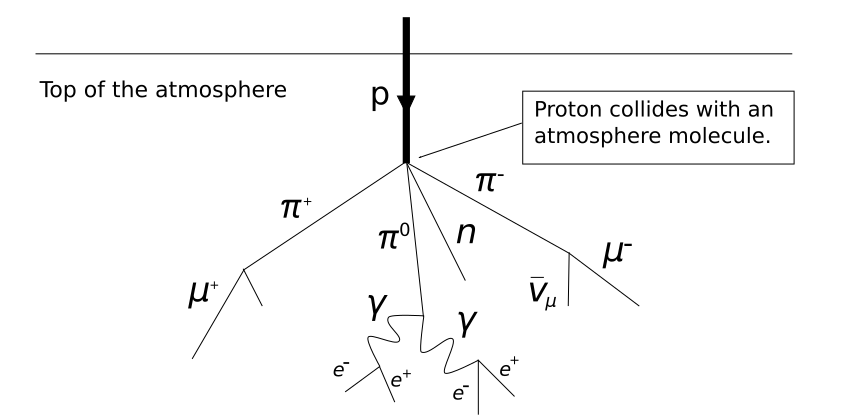
\includegraphics[width=4.5 in]{particleshower}
	\caption{A typical shower}
%%%%%%%%
\end{wrapfigure}
 energetic than --- those deliberately produced in colliders at e.g. CERN and FermiLab. Muons are both generated directly and indirectly (via decay of charged mesons), and often carry relativistic amounts of kinetic energy. Some muons will scatter towards earth, gradually losing energy as they interact with matter in their descent.


High-energies are crucial to muon detection at sea level: the mean muon lifetime in vaccuum is only $\sim 2.2 \mu $s, as measured in the rest frame; therefore, their ability to reach earth's surface depends on time-dilation. This experiment is actually a direct confirmation of special relativity, since you will measure both the arrival of muons and their lifetime.
\begin{QQP}[]
{ If muons are produced $18.3$ km above Earth's surface, how fast must they travel to reach earth's surface within $2.2 \mu $s, ignoring time dilation? Does this seem reasonable? }
\end{QQP}
\subsection{Decay}
When muons decay, they produce an electron-neutrino as well as an electron or positron depending on the charge species. The neutrino, which only interacts with matter weakly and has negligible mass, is undetectable and will likely escape the solar system (possibly the galaxy). The electron (positron), however, will be detectable via the electromagnetic force, and will usually be relativistic as muons are approximately $200$ times more massive.

\begin{QQP}[]
{ If a muon at rest decays, by conservation of energy, what is the maximum velocity of the resultant electron?  }
\end{QQP}

\subsection{Detection}
In this experiment, muon detection relies on the particle's ability to stimulate photon emission inside of your fluor-doped plastic scintillating material via scattering. Scattering occurs when \textit{any} charged particle enters the scintillator and interacts with the molecules via the Coulomb force, imparting a part of its kinetic energy into the material. When some of this energy is transferred to fluor electrons, they are briefly promoted to a highly excited state. As these electrons spontaneously transition back to equilibrium, with a mean excited lifetime of a few nanoseconds, the difference in energy is emitted as a photon. Typically one photon per $100$ eV of deposited energy is produced, with a wavelength in the blue to near-UV spectrum. The photons which reach the PMT are then amplified and converted into a voltage by the photoelectric effect.
\begin{QQP}[]
{ Physics comprehension question }
\end{QQP}

Muons have two ways of participating in scattering: they can scatter themselves directly, or their decay products may scatter. 

\subsection{Signal Management}
I'll discuss proportinality w/ particle energy and some basic stuff about the equipment that will help them understand how their filtering works
\begin{QQP}[]
{ Physics comprehension question }
\end{QQP}

\newpage
\section{Saftey}
Please don't electrocute yourself

\newpage
\section{Theory and Models}
\subsection{Particle Decay and Arrival: Poisson Statistics}
As is true for all fundamental particles, to the best of our knowledge muon decay is governed exactly by Poisson Statistics. That nature chose this decay law is astonishing, since Poisson processes, a kind of Markov process, may be regarded as the simplest random process. In addition to decay, the arrival of muons into your detector is also described by Poissonian statistics. This section will introduce the mathematics of working with Poisson processes. 
\medskip

\subsection{Mathematically Describing Random Processes}
\vspace{-1cm}
\begin{wblurb}[r][0.44][Probability: Markov Processes and Poisson Statistics]{21}
{
  When  we talk about a \textbf{random process}, we are referring to a process in which some \textbf{events} happen at random intervals drawn from some probability distribution. Events can be, for example, a die rolling a one, a person clicking an ad of a social media site, or in our case a muon decay. 

\medskip
We say a process is \textbf{Markov} if the probability of an event happening is independent of the history or timing of events which have already occurred; we say that the process is \textbf{memory-less} and depends only on the current state of the system. Dice are memory-less because the probability of rolling a number is independent of the results of previous rolls. A dynamical system of one particle whose state is described by its position, but with a random external force that depends on its velocity is \textbf{Non-Markov}. If we instead describe the state of the particle using \textit{both} its position \textit{and} its velocity, greatly increasing the number of possible states in the system, the process is again Markov.
\medskip 

A \textbf{Poisson process} is a simple Markov process such that events happen at random, but at a constant average \textbf{rate}. A canonical example of this would be birth and death processes: to a good approximation, birth and death happen at a rate roughly proportional to the population size, which can be considered as the state of the system.}
\end{wblurb}
\vspace{1cm}

When dealing with random processes, our ultimate goal is to convert our basic knowledge of a given system into probabilistic predictions. A system is typically characterized by the possible \textbf{states} it can be in -- e.g. a state with $1, 2, 3 \dots n$ particles detected -- and the \textbf{events}, or transitions, which move the system between each state -- e.g. the process of a particle arriving in your detector, thus taking you from a state $n$ to a state labeled by $n+1$. 

Probability enters our description of our system through events: for any interval of time, there is a probability that an event occurs which changes the state of our system, taking it from say state $A$ to state $B$. We can write this as $p_{A \RA B}(t'-t)$. 

When we know the inital state, our goal is to predict the probability of being in various states at some later time, $P_{state}(t)$ based on the events that could have happened. Mathematically, if we start in state $A$ at $t_1$ and would like to know the probability of being in state $B$ at $t_2$, we are calculating:

\begin{align**}
P_{B}(t_2) &= \l(\text{P of } A\RA B \text{ in } (t_1,t_2)\r) \times (\text{P of being in state } A \text{ at } t_1 )\\
&= p_{A\RA B}(t_2-t_1) P_A(t_1)
\end{align**}


A Poisson process involves the simplest kind of event,  mathematically speaking -- it is an event has a fixed average rate that it occurs. If the rate that the event happens is $r$, we define a Poisson event by
\begin{align**}
p_{A\RA B}(\delta t)= r \delta t
\end{align**}
where $\delta t$ is a very short time interval. 
\bigskip 

\subsubsection{Modeling Particle Arrival}

%Here I'll extend the math I derived in the decay portion by introducing them to calculating things like the variance in muon arrival, the full Poisson distribution with $k$ events etc., and how statistical quantities/error change with the number measured events. They should be able to fit not only their average muon/sec but also the variance they see in this data. While the model is simplistic, of course, it will help them understand what "acceptable" data looks like! There might also be a calculation that can help them identify contamination by electrons?

%For a particle created at $t=t_0$, with Poissonian decay rate $r$, the probability that it has decayed by a time $t$ is then written as the probability that decay has happened in the interval $(t_0,t)$ times the probability that the particle is present at $t_0$ (this is unity, since we demand it was created at this time!)

Particle arrival is well modeled by a Poisson process and, due to its simplicity, it will be the first process we cover. The possible states of the system are simply labeled by the number of particles which have arrived in our detector since we started counting, and their probabilities at a time $t$ are : $P_0(t), P_1(t), P_2(t), \dots P_{\# particles}(t)$. We have one single Poissonian \textit{event} -- arrival -- which takes the system from state with $n$ particles detected to a state with $n+1$, that occurs during some time interval with probability $p_{n|n+1}(t_0,t_1)$.

Let's say we turn on our particle detector at $t_0=0$. From our diligent research, we know that, on average, a particle should arrive at our detector with an average rate $a$. We want to know the probability that no particles have arrived by $t$. How do we deduce this?

The quantity we are after is $P_0(t_f)$. However, this probability depends on the state of the system--namely the probability that a particle wasn't detected yet -- \textit{immediately before} $t$:
\begin{align**}\label{qeq}
P_0(t) =  p_{0|0}(t_f,t_f -\delta t)P_0(t-\delta t)
\end{align**}


For very short intervals, this is simply:

\begin{align**}\label{qeq2}
P_0(t) = (1- a \delta t) P_0(t-\delta t)
\end{align**}

\begin{QQP}[]
{ Explain, in words, what equation equation \ref{qeq} says. Explain where the $(1-a\delta t)$ comes from in equation \ref{qeq2}}
\end{QQP}
Now, since time is continuous\footnote{as far as we know!}, we'll need to take $\delta t \RA 0$. If we rearrange our equation, we see that this limit results in the definition of a derivative:
\begin{align**}
\lim_{\delta t \RA 0}\frac{P_0(t)-P_0(t-\delta t)}{\delta t}&=\\
 \frac{d }{d t}P_0(t) &= -a P_0(t)
\end{align**}
Who's solution is 
\begin{align**}
P_0(t) = P_0(0)e^{-a t}
\end{align**}
What about $P_0(0)$? At $t=0$ we had turned on our detector, so the probability of having not detected a particle is simply $P_0(0)=1$!

Now let's ask for the probability that we've detected exactly one particle by time $t$. The process is similar: first we reason that the probability of having detected one particle at $t$ depends on the probabilty of possible states at $t-\delta t$:
\begin{align**}
P_{1}(t) &=p_{1|1}(t,t-\delta t) P_{1}(t) + p_{1|0}(t,t-\delta t)P_{0}(t-\delta t)\\
&= (1- a \delta t) P_{1}(t) + a\delta t P_{0}(t-\delta t)
\end{align**}
We can again rearrange this and take the continuum limit, but we now have a new term on the right:

\begin{align**}
\frac{d}{dt}P_{1}(t)= -a\l(P_1(t) - P_0(t)\r)
\end{align**}
Luckily, we just solved for this! Plugging in $P_0(t)= e^{-a t}$ and solving the O.D.E., we arrive at

\begin{align**}
P_1(t) = at e^{-at}
\end{align**}

We leave it as an excercise to the reader to prove the following famous (and useful) formula:

\begin{QEQ}[title={\normalsize Probability of Detecting $n$ Particles After a Time $t$}]
\begin{align**}
  P_{n}(t)=\frac{(at)^{n}}{n!}e^{-at}
 \end{align**}
\end{QEQ}


\bigskip 
\subsection{ Modeling the Decay of a Single Muon}
\bigskip 

A Poisson process describes the probability that an event happens in an \textbf{interval} of time. The probability is denoted by $p_{event}(t_1,t_0)$ where $(t_0,t_1)$ is the interval of interest. Since the average rate, $r$, is \textit{constant}, we have that, for a very small interval $(t_0+\delta t,t_0)$:
\begin{align**}
 p_{event}(t_0+\delta t,t_0) &= r(\l[ t_0+\delta  t\r] -t_0) 
\\ &\overset{\delta t \sim 0}{=}r\delta t  
\end{align**}

Events are what change the state of a system, and typically our end goal is to understand the probability of being in given state at some time $t$, $P_{state}(t)$. For systems where events change the number of particles in a system, these states are typically labeled by the number of particles, $P_n$. In the case of the decay of a single particle, there are two possible states: one in which the particle exists with probability denoted $P_1$, and the state in which it is absent, with probability denoted $P_0$. We have one single Poissonian event -- decay -- which takes the system from state $1$ to state $0$, that occurs during some time interval with probability $p_{0|1}(t_0,t_1)$
\bigskip 

 For a particle created at $t=t_0$, with Poissonian decay rate $r$, the probability that it has decayed by a time $t$ is then written as the probability that decay has happened in the interval $(t_0,t)$ times the probability that the particle is present at $t_0$ (this is unity, since we demand it was created at this time!)

\begin{align**}
P_0(t)&=p_{0|1}(t,t_0)P_1(t_0)\\
&=p_{0|1}(t,t_0)
\end{align**}

Note that the subscripts -- which specify a conditional probability -- naturally link two states with the sharing the same index similar to matrix multiplication\footnote{ These are referred to as Transition Matrix Elements in the theory of Markov Processes, and describe the likelyhood of \textit{transitioning} from one state to another. Quite generally, all Markov processes can be modeled as a matrix acting on a vector who's entries are probabilities to be in a given state. For more information on working with}. Like above, the probability of decay in a very small time interval after creation at $t_0$ is given by: $p_{0|1}(t_0+\delta t,t_0)= r\delta t $, so that for a short time

\begin{align**}
P_0(t_0+\delta t) = r\delta t.
\end{align**} 

Similarly, it will be useful to rewrite this in terms of the probability that a decay does not occur, i.e. that the muon is still present. Since the probabilities just add to unity, this is just:

\begin{align**}
P_{1}(t_0 +\delta t) &\equiv p_{1|1}(t_0+\delta t,t_0) P_1(t_0)\\
&= 1-P_{0}(t_0+\delta t)= 1- r\delta t \end{align**}


For our experiment, we care about the state of the muon at a general time $t$. In particular, let's evaluate the probability that our muon, created (or observed) at $t_0=0$ is still present at $t+\delta t$. Following the same logic as above we can write the probability of having a muon at $t+\delta t$ as the probability of having a muon at $t$ times the probability that it does not decay in the short interval of length $\delta t$
	\begin{align**}
	P_1(t+\delta t)&=p_{1|1}(t+\delta t,t)P_1(t)\\
	&= (1-r\delta t)P_1(t)
	\end{align**}
Rearranging this equation and taking the limit $\delta t \RA 0$ (exercise), we obtain the following differential equation:
	

	\begin{align**}
	\d_t P_{1}(t) = -r P_{1}(t)
	\end{align**}
	
Since we know the muon is present at $t=0$, we demand that $P_1(0)=1$, and this can be integrated to the solution


	\begin{align**}
	\boxed{P_{1}(t)= e^{-rt}}
	\end{align**}


This equation describes a probability distribution over time, and is the basis of all calculations used in the muon lifetime experiment. Be sure you understand it! 


%\begin{wrapfigure}[8]{l}[0pt]{0.35\textwidth}
%\blurb[width=0.35\textwidth,center,Probability: Averages and Variances]
%{
%In probability, averages (or \textbf{expectation values}) are computed by summing over the values of a random variable multiplied by the probability of that value:
%
%$\langle x\rangle \equiv \sum_{i}x_i P_i$ 
%  
%As an example, for a regular die, the expecation value of a roll is (I might make this a side info box w/ picture):
%  
%$\langle \+{roll}\rangle = \l(1\r)\l(\frac{1}{6}\r)+\l(2\r)\l(\frac{1}{6}\r)+\l(3\r)\l(\frac{1}{6}\r)+\l(4\r)\l(\frac{1}{6}\r)+\l(5\r)\l(\frac{1}{6}\r)+\l(6\r)\l(\frac{1}{6}\r) = 3.5$	
%  	}
%\end{wrapfigure}

\bigskip

  


  	
  	
\textbf{\sc \underline{Lifetime.}}  We now illustrate how to perform an important calculation: the \textbf{average lifetime} of a muon. 
For the case of the average lifetime, our random variable is a small interval of time around $t$, $(t,t+\delta t)$, and the probability is the probability that a decay happens in that specific interval $p_{0|1}(t,t+\delta t) P_1(t)$.  
	\begin{flalign*}
	&& \langle t\rangle &= \sum_{t=0}^{\infty} t \times p_{0|1}(t,t+\delta t) P_1(t)
	\\ && &=\sum_{t=0}^{\infty} t  r e^{-r t}\delta t
	\\&& & = r \int_{0}^{\infty} t  e^{-rt }dt &\llap{Continuum Limit  \hspace{1cm}}
	\end{flalign*} 
Thus the expectation value for the time of decay is
	\begin{align**}
	\tau \equiv \langle t\rangle_{decay} =\frac{1}{r}
	\end{align**}

Note that the expectation value is the averaged measured value obtained by an experiment in the (unrealistic) limit that the number of recorded events goes to infinity. You will see fluctuations in your live data, and your final result will not exactly match the accepted value. You should compare these fluctuations and deviations with the expected variance, which can be computed similar to above, taking into account the number of measurements you have performed.
\subsubsection{Advanced: Modeling the Decay of Multiple Muons}
TA Note: Here I'll briefly show how to get the distribution for multiple muons since there are many ways to do this incorrectly. Follow up questions on muon arrival will actually demonstrate that this isn't so important since its unlikely two or more muons will be in the detector simultaneously-- but it's here if a student wants to be overly meticulous and calculate an error from it. I'll also discuss charge averaged lifetimes here.

\textbf{Multiple Identical Muons.} We now examine the case that rather than a single muon, we have multiple muons at time $t_0=0$ with independent decay. In this case, we will compute the probability that $1$ out of the initial $n_0$ decay in some small time interval, $P_{n_0-1}(t_0,t_0 +\delta t)$. Since they are independent, for infinitesimal $\delta t$
\begin{align**}
P_{n_0-1}(\delta t) =  p_{n_0-1|n_0} = {n_0\choose 1} r \delta t = n_0 r\delta t
\end{align**}
And the probability that none decay is then
\begin{align**}
P_{n_0}(\delta t) = p_{n_0|n_0}=(1-n_0 r\delta t)
\end{align**}

Following the previous section, we compute the probability to have $n$ muons at a given time by considering the probability at $t+\delta t$
\begin{align**}
P_n(t+\delta t) = P_n(t)(1-nr\delta t) + P_{n+1}(t)(n+1)r \delta t
\end{align**} 
Which gives the differential equation for general $n$:
\begin{align**}
\d_t P_n(t_0,t) = -nrP_n(t)+ (n+1)rP_{n+1}(t)
\end{align**}

The new term here comes from the fact that the state with $n$ muons could come from a decay in the previous time interval. Because of this term, we will have to solve this equation recursively. For $n=n_0$, where $n_0$ is the maximum number of particles set by the initial condition, $P_{n_0+1}(t)=0$ and we get 
\begin{align**}
P_{n_0}(t) =  e^{-n_0 rt}
\end{align**}
For $n=n_0-1$, we can then identify  $P_{n_0}(t)=e^{-n_0 rt}$ leading to the inhomogenous ODE:
\begin{align**}
\l[ \d_t   +(n_0-1)r \r]P_{n_0-1}(t)= n_0 re^{-n_0 rt}
\end{align**}
Which integrates to the solution
	\begin{align**}
	P_{n_0-1}(t)=n_0 e^{-n_0 rt} (e^{ rt} -1)
	\end{align**}
We leave it as an exercise to prove that for general $n=n_0 -k$
\begin{align**}\label{generalk}
P_{n_0-k}(t)= \frac{n_0!}{k!(n_0-k)!}(e^{rt}-1)^k e^{-n_0 rt}
\end{align**}

A familiar result emerges if we use the above distribution to determine the average number of muons at time $r$:
\begin{align**}
\bar N(t) \equiv \langle n_0-k\rangle(t) &= \sum_{k=0}^{n_0}\l(n_0-k\r)\frac{n_0!}{k!(n_0-k)!}(e^{rt}-1)^k e^{-n_0 rt}\\
& = n_0ksdflka
\end{align**}

\textbf{Muons of Different Charge Species.}
\subsection{Corrections: Relativistic Energies and Scattering}
Quick review of time dilation and an overview of how to account for energy loss due to scattering. Will mostly borrow from the previous manual.

\newpage
\section{Experimental Procedure Guide}
\newcommand{\chk}{{\large $\Box \;$}}
You must research and collect data (with reported error) and record your sources for this lab. Find accepted values for the following quantities to which you will compare your final results against:
 
\begin{center}
\begin{tabular}{ l@{\hspace{0.5in}} l}
 \chk Muon lifetimes (note charge species) & \chk Mean muon production height \\ 
 \chk Average muon flux at sea level  & \chk SR-90 $\beta$-- energy spectrum \\  
 \chk Average muon energy at sea level & \chk Flux Angular Dependence Model
\end{tabular}
\end{center}

Prior to connecting any equipment, take time to identify and collect the following components which will be used throughout the lab. If you cannot find an item, ask your TA for assistance.
\medskip

\begin{center}
\begin{tabular}{ l@{\hspace{0.5in}} l@{\hspace{0.5in}} l }
 \chk 2 Scintllators & \chk NIM rack & \chk Oscilloscope \\ 
\chk 2 PMTs & \chk Cables & \chk Serial connection to PC \\  
 \chk FGPA Timer & \chk Terminators & \chk Function Generator \\
 \chk Amplifier & \chk Splitter & \chk Multimeter    
\end{tabular}
\end{center}
\medskip
The first section of this guide walks you through understanding your equipment. It should take you no longer than one week to complete. After completing this part of the lab, you will design two experiments that measure the angular flux of muons and muon lifetime. The guide sections corresponding to these measurements do not tell you how to accomplish this; they provide a list of useful questions who's answers should be important to the design and analysis. You are not required to complete these questions (unless specified), but it is strongly recommended that you do.
\subsection{Understanding your Equipment}
\subsubsection{Detector Basics}
\begin{enumerate}
\item After completing Prelab question (Qnumber: this will explain terminator), directly connect the wand PMT to your oscilloscope appropriately, finding scale and trigger settings such that you obtain clear signals. Figure out what these signals represent. What are their widths and why? Do the signals have different heights? Why?
\item Route the PMT output through your amplifier and then into the Oscilliscope. Verify that the signals look as expected.
\item Split the amplifier output into both the oscilloscope and the NIM module. Put the NIM module into count mode. Do the counts match what you see on the oscilloscope? If not, figure out why.
\item Record the counts obtained for a $100$s interval, and compare the result to the expected muon flux based on your scintillator area. What needs to be adjusted, and in what direction, to match your expectations? Repeat this until you think your settings are satisfactory.
\item Put an SR-90 source on the wand PMT and record counts for $100$s. Does this change your count rate in a statistically significant way? What does this mean about your ``muon counts"?
\item Continue to adjust your discriminator until you are confident that most counts are due to muons. It will be helpful to plot the counts obtained for both ambient and SR-90 contaminated data as a function of discriminator setting. Is it better to filter out some muon signals or to accidentally count some high-energy electrons? Why?
\item Split the PMT output into two cables of different length. Using the oscilloscope, estimate the differential signal latency. What causes this?
\end{enumerate}
\subsubsection{Advanced Techniques}
\begin{enumerate}
\item Measure the gain of the 2-stage amplifier using a sine wave.
 Apply a 100kHz 100mV peak-to-peak sine wave to the input of the electronics box
input. Measure the amplifier output and take the ratio Vout/Vin. Due to attenuation
resistors inside the electronics box inserted between the amplifier output and the front
panel connector, you will need to multiply this ratio by the factor 1050/50 = 21 to
determine the real amplifier gain..\\
Q: Increase the frequency. How good is the frequency response of the amp?\\
Q: Estimate the maximum decay rate you could observe with the instrument.
\item Measure the saturation output voltage of the amp.
 Increase the magnitude of the input sine wave and monitor the amplifier output.\\
 Q: Does a saturated amp output change the timing of the FPGA? What are the
implications for the size of the light signals from the scintillator?
\item Examine the behavior of the discriminator by feeding a sine wave to the box input and
adjusting the discriminator threshold. Monitor the discriminator output and describe its
shape.
\item Measure the timing properties of the FPGA:
\begin{enumerate}
 \item Using the pulser on the detector, measure the time between successive rising edges
on an oscilloscope. Compare this number with the number from software display.
 \item Measure the linearity of the FPGA:
 Alter the time between rising edges and plot scope results v. FPGA results;
 Can use time between 1 $\mu$s and 20 $\mu$s in steps of 2 $\mu$s.
 \item Determine the timeout interval of the FPGA by gradually increasing the time between
successive rising edges of a double-pulse and determine when the FPGA no longer
records results;\\
 Q: What does this imply about the maximum time between signal pulses?
 \item Decrease the time interval between successive pulses and try to determine/bound the
FPGA internal timing bin width.\\
 Q: What does this imply about the binning of the data?\\
 Q: What does this imply about the minimum decay time you can observe? 
\end{enumerate}
\item Adjust (or misadjust) discriminator threshold.
Increase the discriminator output rate as measured by the scope or some other means.
Observe the raw muon count rate and the spectrum of "decay" times. (This exercise needs
a digital scope and some patience since the counting rate is “slowish.”)

\item What HV should you run at? Adjust/misadjust HV and observe amp output. (We know
that good signals need to be at about 200 mV or so before discriminator, so set
discriminator before hand.) With fixed threshold, alter the HV and watch raw muon count
rate and decay spectrum.
\item Connect the output of the detector can to the input of the electronics box. Look at the
amplifier output using a scope. (A digital scope works best.) Be sure that the scope
input is terminated at 50$\Omega$. What do you see? Now examine the discriminator
output simultaneously. Again, be certain to terminate the scope input at 50$\Omega$. What do
you see?
\item Set up the instrument for a muon lifetime measurement.
 Start and observe the decay time spectrum.\\
 Q: The muons whose decays we observe are born outside the detector and therefore
spend some (unknown) portion of their lifetime outside the detector. So, we never
measure the actual lifetime of any muon. Yet, we claim we are measuring the lifetime of
muons. How can this be?
\item Fitting the decay time histogram can be done with the included fitter or with your own.
\item From your measurement of the muon lifetime and a value of the muon mass from
some trusted source, calculate the value of Fermi coupling constant GF. Compare your
value with that from a trusted source.
\item Using the approach outlined in the text, measure the charge ratio $\rho$ of positive to
negative muons at ground level or at some other altitude.
\item Following the approach in the manual, measure the muon stopping rate at two
different elevations and compare predictions that do and do not assume the time dilation
effect of special relativity. 
\end{enumerate}
\subsection{Angular Distribution of Muon Flux}
Design an experiment that measures the angular distribution of muon flux.
When measuring the amplitude and directionality of the muon flux, you will interface two scintillator/PMT apparatuses directly with the rack of equipment housing the NIM electronics. Your goal is to quantify the rate and directionality with respect to the zenith, of incoming cosmic-ray muons. 

You are encouraged to talk over the following discussion questions with your partner and TA, especially if you find yourself conceptually stuck in working out a good procedure:

{\setstretch{1.0}
\begin{itemize}
\item What is a coincidence measurement? Ideally, what will physically occur, what signals will be produced, and how will coincidence be determined?
\item When a particle is detected, does its energy change?
\item How far apart do you think your detectors should be?
\item Do you think the building has an effect on the rate and angular dependence of flux?
\item What kinds of events might produce ``false signals" ? Is there a way you can use your equipment to measure the rate of these ``false signals"? How important are these in this measurement? In which way, if any, will they skew mean? How will they affect variance?
\item Why should muon flux depend on the angle? What changes as the angle goes from vertical to horizontal?
\item Do you think you can measure the absolute muon flux at a given angle to a high degree of accuracy? Why or why not?
\item Does the answer to the previous question impact your ability to estimate the differential flux as a function of angle?
\item Are there any places in your signal pathway that latency might be important? 
\item Can you demonstrate that muons are coming from the sky, rather than the earth?
\end{itemize}}

Once you've progressed to a point where you have developed a plan --- by fiddling with the equipment and researching concepts as necessary --- run it by your TA. Be prepared to justify the details of your set-up qualitatively, quantitatively  and with data as appropriate.


\subsection{Muon Lifetime}
Design an experiment that measures the muon lifetime. This experiment will utilize the large cylindrical detector and the TeachSpin module to acquire data. The latter is a ``black box" and is strictly provided for convenience --- it digitizes your count data automatically so you can perform long runs. You should consider concurrently using the wand detector and NIM bin  setup to verify it is working as expected. 


You are encouraged to talk over the following discussion questions with your partner and TA, especially if you find yourself conceptually stuck in working out a good procedure:


{\setstretch{1.0}
\begin{itemize}
\item What are you trying to measure in this part of the experiment? Ideally, what will physically occur, what signals will be produced, and how will a decay be determined?
\item What do you think the TeachSpin box does? Can you demonstrate this?
\item What things need to be true about the muon in order for its decay to be detected?
\item What, roughly, is the time resolution of your apparatus? I.e. how far apart to signals need to be in order to identify them as separate events? 
\item What kinds of events might produce ``false signals" ? Is there a way you can use your equipment to limit contamination by these ``false signals"? How important are these in this measurement? In which way, if any, will they skew mean? How will they affect variance?
\item What information do you need to calibrate your discriminator to filter out the aforementioned signals? How does the experiment's physical environment and your equipment's detection efficiency change your expectations for baseline muon flux? Does this matter?
\end{itemize}
}
Once you've progressed to a point where you have developed a plan --- by fiddling with the equipment and researching concepts as necessary --- run it by your TA. Be prepared to justify the details of your set-up qualitatively, quantitatively  and with data as appropriate.
\newpage
\section{Pre-Lab Work}
You will not be permitted to begin the experiment until the safety questions are completed and correct. Ideally all questions should be completed prior to the portion of lab that they address. You may need to look up (with source stated) reported numerical values of various quantities or numerically evaluate some equations to answer questions.

\subsection{Saftey (5 points)}
\begin{enumerate}
\item List all safety concerns with a one to two sentence description of how you will avoid placing you and your partner(s) in danger
\end{enumerate}
\subsection{Theory (10 points)}
\begin{enumerate}
\item Assume the muon decay rate is $0.45 \+{decays}/{\mu s}$. What is the probability that a muon at rest in your detector decays within a time interval of $20 \mu s$?
\item In practice, two signals in your detector can only be resolved if there is sufficient time between their arrivals--- this means that there is lower cut-off, $\Delta t_{\+{min}}=t_{\+{decay}}-t_{\+{arrive}}$, for two subsequent signals to be counted. Find a value of $\Delta t$ such that there is a 1\% probability of a decay. How does this compare to your actual resolution?
\item Why does the time a muon traveled prior to entering your detector not matter? Defend this mathematically.
\item Particle decay rates are always reported in terms of the muon rest frame. Calculate the probability of decay as a function of time for a relativistic muon traveling at speed $v$ in the lab frame. Calculate the measured lifetime.
\item Using the results from the above question and assuming a perfect vacuum, what is the average energy of a muon which reaches your detector if they are created a height R above the detector? What is the lowest muon energy such that 5\% reach the detector?
\item What is the probability that two muons enter a $1\+{cm}^{2}$ detector at sea-level in a $20\mu$s time interval? How about three? Is it ok to assume that there is only ever one muon in your detector at a time? You will need to look up sea-level muon flux rate.
\item Verify that equation \eqref{generalk} is normalized for all $t>t_0$
\item Look up the density of air in the atmosphere and estimate the energy loss of muons between their origin and sea-level. You may use mathematical software to integrate the equations as necessary. 
\end{enumerate}

\subsection{Apparatus (10 points)}
\begin{enumerate}
\item Draw a labeled diagram of your signal pathway (for both experiments) starting with muon production. For each device in the pathway, explicitly identify the input and output with units as appropriate. Which devices do you have direct control over (e.g. choosing a threshold), and what is your uncertainty? What do you expect to be the largest source of uncertainty and why?
\item Circuit diagram question about terminator impedance matching
\end{enumerate}
\newpage

\appendix
\section{Solution Manual}
\begin{align**}
sdfsd
\end{align**}





\end{document}
%
% ****** End of file apstemplate.tex ******

